\PassOptionsToPackage{no-math}{fontspec}
% texlate: native XeTeX font and PDF-driver capabilities
\AddToHook{package/microtype/after}{%
\DeclareMicrotypeSet{texlate-native}{encoding={TU,EU1,EU2}}%
\UseMicrotypeSet[protrusion]{texlate-native}%
}
% breakurl already has a native-PDF branch; limit its PDF-mode override to loading.
\AddToHook{package/breakurl/before}{%
\RequirePackage{xkeyval,ifpdf}%
\let\TeXlateSavedIfpdf\ifpdf\let\ifpdf\iftrue
}
\AddToHook{package/breakurl/after}{\let\ifpdf\TeXlateSavedIfpdf}
% This class's optional arXiv check assumes every non-pdfTeX engine writes DVI.
\PassOptionsToClass{nopdfoutputerror,allowfontchangeintitle}{quantumarticle}
% Embedded PostScript can silently disappear with restricted XeTeX drivers.
% Record actual drawing operations; merely loading an unused package is harmless.
\AddToHook{package/pstricks/after}{%
\ifcsname pst@object\endcsname
\expandafter\let\expandafter\TeXlatePstObject\csname pst@object\endcsname
\expandafter\def\csname pst@object\endcsname#1{%
\typeout{TeXlate-PostScript-object: #1}\TeXlatePstObject{#1}}%
\fi
}
% \DeclareUnicodeCharacter is pdfTeX/inputenc-only and undefined under XeTeX,
% but e-print preambles still call it (2501.14787). Emulate via the lccode
% idiom: make the code point an active char expanding to the replacement.
\providecommand{\DeclareUnicodeCharacter}[2]{%
\begingroup\lccode`\~="#1\relax
\lowercase{\endgroup\catcode`~\active\protected\def~}{#2}}
\documentclass[sigconf]{acmart}
\makeatletter\let\liningnums\@undefined\makeatother
\usepackage[fontset=fandol,UTF8]{ctex}  % [texlate injected]
% texlate: twin named-dest for shared-counter theorems
\makeatletter
\def\TeXlate@thmtwin{%
  \@ifundefined{MakeLinkTarget}{}{%
  \@ifundefined{@currentcounter}{}{%
  \@ifundefined{theH\@currentcounter}{}{%
    \ifx\@currenvir\@currentcounter
      \@ifundefined{alias@ctr@\@currenvir}{}{%
        \edef\TeXlate@twin{\csname alias@ctr@\@currenvir\endcsname}%
        \TeXlate@emit}%
    \else
      \@ifundefined{the\@currenvir}{}{%
        \let\TeXlate@twin\@currenvir
        \TeXlate@emit}%
    \fi}}}%
}%
\def\TeXlate@emit{%
  \begingroup
  \let\TeXlate@save\@currentHref
  \edef\TeXlate@name{\TeXlate@twin.\csname theH\@currentcounter\endcsname}%
  \MakeLinkTarget*{\TeXlate@name}%
  \global\let\@currentHref\TeXlate@save
  \endgroup}%
\AddToHook{cmd/@begintheorem/before}{\TeXlate@thmtwin}%
\AddToHook{cmd/@opargbegintheorem/before}{\TeXlate@thmtwin}%
\makeatother

% texlate: math fallback via dedicated symbol fonts
\ifdefined\Umathcode
\makeatletter
\DeclareFontFamily{TU}{texlatecjk}{\hyphenchar\font\m@ne}
\DeclareFontShape{TU}{texlatecjk}{m}{n}{<->"[FandolSong-Regular.otf]"}{}
\DeclareFontShape{TU}{texlatecjk}{b}{n}{<->"[FandolSong-Bold.otf]"}{}
\DeclareFontShape{TU}{texlatecjk}{bx}{n}{<->ssub*texlatecjk/b/n}{}
\DeclareFontShape{TU}{texlatecjk}{m}{it}{<->ssub*texlatecjk/m/n}{}
\DeclareFontShape{TU}{texlatecjk}{m}{sl}{<->ssub*texlatecjk/m/n}{}
\DeclareFontShape{TU}{texlatecjk}{b}{it}{<->ssub*texlatecjk/b/n}{}
\DeclareFontShape{TU}{texlatecjk}{bx}{it}{<->ssub*texlatecjk/b/n}{}
\DeclareFontShape{TU}{texlatecjk}{bx}{sl}{<->ssub*texlatecjk/b/n}{}
\DeclareSymbolFont{texlatecjk}{TU}{texlatecjk}{m}{n}
\SetSymbolFont{texlatecjk}{bold}{TU}{texlatecjk}{b}{n}
\def\TeXlate@mathmap#1#2-#3;{\count@="#2\relax
  \@whilenum\count@<"#3 \do{\Umathcode\count@="0 #1 \count@\advance\count@\@ne}}
\TeXlate@mathmap\symtexlatecjk 4E00-9FFF;
\TeXlate@mathmap\symtexlatecjk 3400-4DBF;
\TeXlate@mathmap\symtexlatecjk 3000-303F;
\TeXlate@mathmap\symtexlatecjk FF00-FFEF;
\TeXlate@mathmap\symtexlatecjk 3040-30FF;
\TeXlate@mathmap\symtexlatecjk F900-FAFF;
\TeXlate@mathmap\symtexlatecjk 2E80-2FDF;
\TeXlate@mathmap\symtexlatecjk 20000-2A6DF;
\TeXlate@mathmap\symtexlatecjk 2A700-2EBEF;
% 非 CJK 带（西里尔人名 Ш/Д/Л、组合符、拉丁扩展）走 Libertinus Serif;
% \IfFileExists 门——otf 缺席则整段不挂, 免把缺字升级成字体加载错误。
% 00D7 ×/00F7 ÷ 是 binop 语义, 普通 ordinary 化会改距, 故带内挖掉。
\IfFileExists{LibertinusSerif-Regular.otf}{%
\DeclareFontFamily{TU}{texlatefb}{\hyphenchar\font\m@ne}
\DeclareFontShape{TU}{texlatefb}{m}{n}{<->"[LibertinusSerif-Regular.otf]"}{}
\DeclareFontShape{TU}{texlatefb}{b}{n}{<->"[LibertinusSerif-Bold.otf]"}{}
\DeclareFontShape{TU}{texlatefb}{bx}{n}{<->ssub*texlatefb/b/n}{}
\DeclareFontShape{TU}{texlatefb}{m}{it}{<->ssub*texlatefb/m/n}{}
\DeclareFontShape{TU}{texlatefb}{m}{sl}{<->ssub*texlatefb/m/n}{}
\DeclareFontShape{TU}{texlatefb}{b}{it}{<->ssub*texlatefb/b/n}{}
\DeclareFontShape{TU}{texlatefb}{bx}{it}{<->ssub*texlatefb/b/n}{}
\DeclareFontShape{TU}{texlatefb}{bx}{sl}{<->ssub*texlatefb/b/n}{}
\DeclareSymbolFont{texlatefb}{TU}{texlatefb}{m}{n}
\SetSymbolFont{texlatefb}{bold}{TU}{texlatefb}{b}{n}
\TeXlate@mathmap\symtexlatefb 0400-04FF;
\TeXlate@mathmap\symtexlatefb 0300-036F;
\TeXlate@mathmap\symtexlatefb 00C0-00D6;
\TeXlate@mathmap\symtexlatefb 00D8-00F6;
\TeXlate@mathmap\symtexlatefb 00F8-017F;
}{}
\makeatother
\fi

% texlate: xeCJK first-use warmup (frontmatter \vbox poison)
\ifdefined\XeTeXversion
\AtBeginDocument{\setbox0=\hbox{字}}%
\fi

% texlate: \t absent from tuenc.def -> TS1 \accent bypasses xeCJK
\ifdefined\UnicodeEncodingName
\DeclareUnicodeAccent{\t}{"0361}
\fi


\usepackage{booktabs} % For formal tables
\usepackage{graphicx}
\usepackage{subfigure}


% Copyright
%\setcopyright{none}
%\setcopyright{acmcopyright}
%\setcopyright{acmlicensed}
\setcopyright{rightsretained}
%\setcopyright{usgov}
%\setcopyright{usgovmixed}
%\setcopyright{cagov}
%\setcopyright{cagovmixed}


% DOI
\acmDOI{10.475/123_4}

% ISBN
\acmISBN{123-4567-24-567/08/06}

%Conference
\acmConference[SIGSPATIAL'17]{ACM SIGSPATIAL conference}{November 2017}{Redondo Beach, California USA} 
\acmYear{2017}
\copyrightyear{2017}

\acmPrice{15.00}


% texlate: fit complete oversized float boxes v1
\usepackage{graphicx}
\begingroup
\makeatletter
\AtBeginDocument{%
\let\texlate@endfloatbox\@endfloatbox
\def\@endfloatbox{%
\texlate@endfloatbox
\def\texlate@figure{figure}%
\def\texlate@figurestar{figure*}%
\def\texlate@table{table}%
\def\texlate@tablestar{table*}%
\let\texlate@floatscope\@empty
\ifx\@currenvir\texlate@figure\def\texlate@floatscope{1}\fi
\ifx\@currenvir\texlate@figurestar\def\texlate@floatscope{1}\fi
\ifx\@currenvir\texlate@table\def\texlate@floatscope{1}\fi
\ifx\@currenvir\texlate@tablestar\def\texlate@floatscope{1}\fi
\ifx\texlate@floatscope\@empty\else
\ifdim\dimexpr\ht\@currbox+\dp\@currbox\relax>\textheight
\edef\texlate@floatwidth{\the\wd\@currbox}%
\edef\texlate@floatheight{\the\dimexpr\textheight-\baselineskip\relax}%
\ifdim\texlate@floatheight>0pt
\typeout{TeXlate-Float-Fit: \@captype\space \csname the\@captype\endcsname; height \the\dimexpr\ht\@currbox+\dp\@currbox\relax; limit \texlate@floatheight}%
\global\setbox\@currbox=\vbox{\hbox to\texlate@floatwidth{\hfil\resizebox*{!}{\texlate@floatheight}{\box\@currbox}\hfil}}%
\fi\fi\fi}%
}
\endgroup
\begin{document}
	\title{这是译文}
	
	\author{Yi Zhu}
	\affiliation{%
		\institution{University of California, Merced}
	}
	\email{yzhu25@ucmerced.edu}
	
	\author{Sen Liu}
	\affiliation{%
		\institution{University of Southern California}
	}
	\email{senliu@usc.edu}
	
	\author{Shawn Newsam}
	\affiliation{%
		\institution{University of California, Merced}
	}
	\email{snewsam@ucmerced.edu}
	
	% The default list of authors is too long for headers}
	\renewcommand{\shortauthors}{Yi Zhu, Sen Liu and Shawn Newsam}
	
	
	\begin{abstract}
		这是译文.
	\end{abstract}
	
	%
	% The code below should be generated by the tool at
	% http://dl.acm.org/ccs.cfm
	% Please copy and paste the code instead of the example below. 
	%
	
	\begin{CCSXML}
		<这是译文~这是译文~这是译文~这是译文~这是译文~这是译文~这是译文~这是译文~这是译文2012>
	\end{CCSXML}
	
	\ccsdesc[500]{Information systems~Spatial-temporal systems}
	\ccsdesc[300]{Information systems~Video search}
	\ccsdesc[500]{Human-centered computing~Geographic visualization}
	\ccsdesc[500]{Human-centered computing~Empirical studies in visualization}
	\ccsdesc[500]{Computing methodologies~Activity recognition and understanding}
	\ccsdesc[500]{Computing methodologies~Video summarization}
	\ccsdesc[500]{Computing methodologies~Supervised learning by classification}
	\ccsdesc[500]{Computing methodologies~Neural networks}
	
	\keywords{这是译文}
	
	\maketitle
	
	\section{这是译文}
	\label{sec:introduction}  这是译文. 
	
	这是译文 (这是译文) 这是译文 \cite{Density_Demsar_2010,Trajectory_Qi_2013,LULC_Activity_Li_2017} 这是译文 \cite{Activity_Aware_Phithakkitnukoon_2010,Mobile_Sagl_2014,Phone_NE_2015,Mobility_Yang_2016,Generative_Yin_2017}. 这是译文.
	
	这是译文.
	
	这是译文 \cite{City_Story_Kling_2012,Twitter_Hawelka_2014}. 这是译文 \cite{Twitter_Hawelka_2014} 这是译文.
	
	这是译文 \cite{Flickr_Kisilevich_2010,VGI_Sun_2013,Magnetism_Paldino_2015,Emotions_Hauthal_2016,Travel_Yuan_2016}. 这是译文.
	
	这是译文 (这是译文) 这是译文.
	
	这是译文.
	
	这是译文 \cite{ucf101,activityNet,KarpathyCVPR14,YouTube_8M_2016} 这是译文 (这是译文) 这是译文.
	
	这是译文:
	
	\begin{itemize}
		\item 这是译文.
		\item 这是译文 $130$ 这是译文 (这是译文) 这是译文.
		\item 这是译文.
		\item 这是译文.
		\item 这是译文.
		\item 这是译文.
		\item 这是译文.
		\item 这是译文.
	\end{itemize}
	
	
	\section{这是译文}
	\label{sec:related_work}  这是译文.
	
	\noindent \textbf{这是译文}  这是译文 \cite{CrandallMapWorld09}, 这是译文 \cite{landuse_yi_sigspatial_2015}, 这是译文 \cite{Haysim2gps08,geolocalization_Gupta_2016}, 这是译文 \cite{3dModelSnavely08}, 这是译文 \cite{Magnetism_Paldino_2015}, 这是译文 \cite{emotion_yi_sigspatial_2016}.
	
	这是译文.
	
	这是译文.
	
	\noindent \textbf{这是译文}  这是译文 \cite{Overhead_Hammoud_2013,Structure_Bodensteiner_2015,event_More_2016,geolocalization_Gupta_2016}.  这是译文.
	
	\noindent \textbf{这是译文}  这是译文 (这是译文) \cite{idtfWang2013} 这是译文 \cite{peng2014action,MIFS2015,dovf_lan_2017} 这是译文 \cite{KarpathyCVPR14,c3d2015}, 这是译文 \cite{twostream2014, wanggoodpractice2015} 这是译文 \cite{tvl1realTime} 这是译文 (这是译文) 这是译文 \cite{wanggoodpractice2015,convTwoStream2016,depth2action,TSN2016,res_two_stream_nips16,diba_tle_2016}. 这是译文.
	
	这是译文 \cite{hidden_zhu_17} 这是译文 \cite{c3d2015}. 这是译文. 
	
	\section{这是译文}
	\label{sec:methodology}  这是译文 \ref{sec:problem_formulation}. 这是译文 \ref{sec:hidden_two_stream_networks}. 
	
	\subsection{这是译文}
	\label{sec:problem_formulation}  这是译文 \ref{sec:introduction} 这是译文 \cite{hidden_zhu_17} 这是译文 \ref{sec:hidden_two_stream_networks}.
	
	这是译文 $8$ 这是译文, \textbf{这是译文}, 这是译文 \textbf{这是译文} 这是译文 \textbf{这是译文} 这是译文 $10$ 这是译文.
	
	\begin{figure}[t]
		\centering
		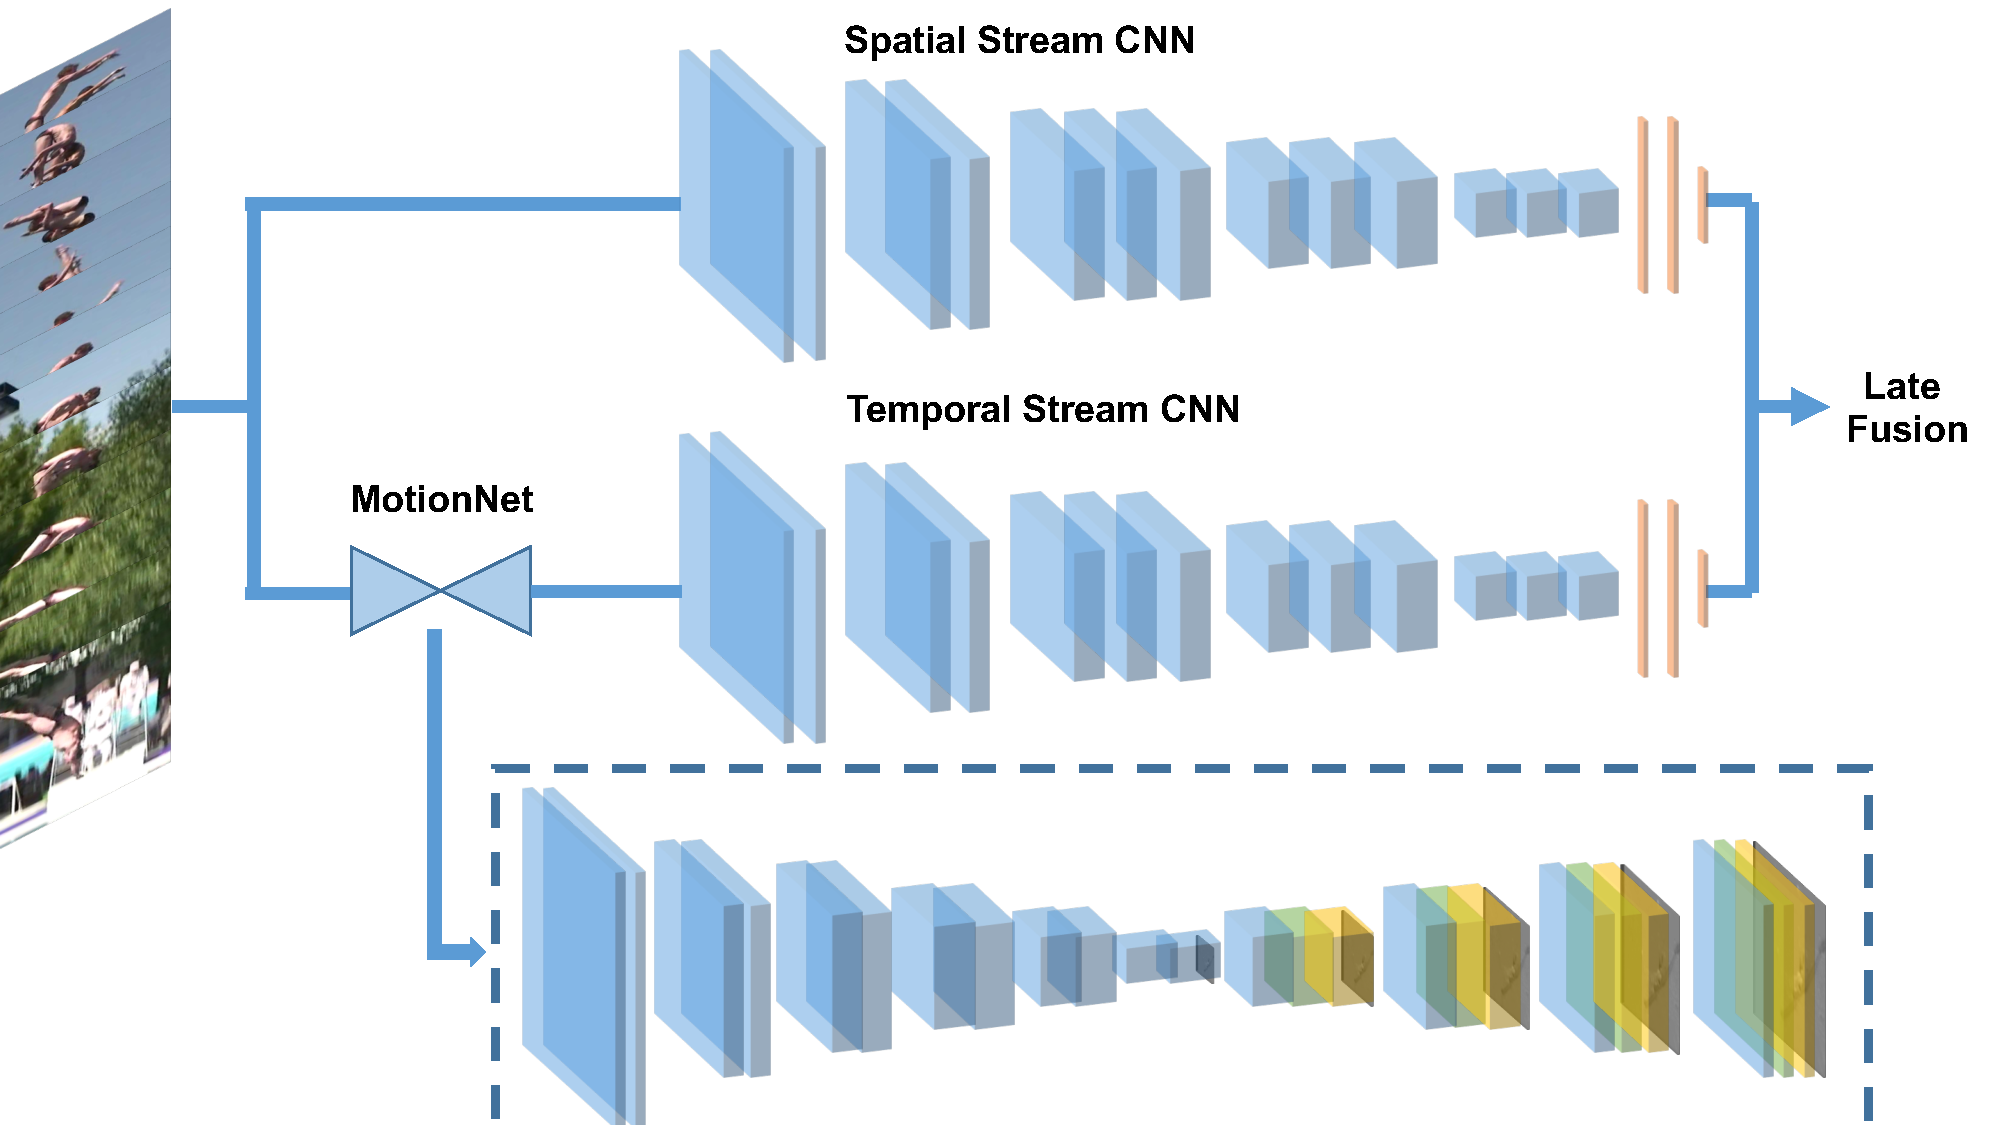
\includegraphics[width=1.0\linewidth,trim=0 0 0 0,clip]{framework_hidden.pdf}
		\caption{这是译文.}
		\label{fig:framework_hidden}
	\end{figure}
	
	\subsection{这是译文}
	\label{sec:hidden_two_stream_networks}  这是译文 \cite{hidden_zhu_17} 这是译文 \cite{twostream2014} 这是译文 \ref{sec:two_stream_networks}. 这是译文 \ref{sec:motionnet}. 这是译文 \ref{sec:stacked_temporal_stream}, 这是译文.
	
	\subsubsection{\textbf{这是译文}}
	\label{sec:two_stream_networks}
	% \noindent \textbf{Two-Stream Networks Recall}
	
	这是译文 \ref{sec:related_work}, 这是译文 \cite{wanggoodpractice2015,convTwoStream2016,depth2action,TSN2016,res_two_stream_nips16,diba_tle_2016} 这是译文 \cite{twostream2014}. 这是译文 (这是译文) 这是译文.
	
	这是译文 $0.065s$ 这是译文 $320\times240$ 这是译文1 \cite{tvl1realTime} 这是译文.
	
	\begin{table}[t]
		\begin{center}
			\resizebox{1.0\columnwidth}{!}{%
				\begin{tabular}{ | c | c | c | c | c | c |  c |}
					\hline
					Name        	&    Kernel & Str & Ch I/O    &    In Res & Out Res   & Input      \\
					\hline		
					conv1 & $3\times3$ & $1$ & $33/64$ & $224\times224$ & $224\times224$ & Frames \\
					conv1$\_$1 & $3\times3$ & $1$ & $64/64$ & $224\times224$ & $224\times224$ & conv1 \\
					conv2 & $3\times3$ & $2$ & $64/128$ & $224\times224$ & $112\times112$ & conv1$\_$1 \\
					conv2$\_$1 & $3\times3$ & $1$ & $128/128$ & $112\times112$ & $112\times112$ & conv2 \\
					conv3 & $3\times3$ & $2$ & $128/256$ & $112\times112$ & $56\times56$ & conv2$\_$1 \\
					conv3$\_$1 & $3\times3$ & $1$ & $256/256$ & $56\times56$ & $56\times56$ & conv3 \\
					conv4 & $3\times3$ & $2$ & $256/512$ & $56\times56$ & $28\times28$ & conv3$\_$1 \\
					conv4$\_$1 & $3\times3$ & $1$ & $512/512$ & $28\times28$ & $28\times28$ & conv4 \\
					conv5 & $3\times3$ & $2$ & $512/512$ & $28\times28$ & $14\times14$ & conv4$\_$1 \\
					conv5$\_$1 & $3\times3$ & $1$ & $512/512$ & $14\times14$ & $14\times14$ & conv5 \\
					conv6 & $3\times3$ & $2$ & $512/1024$ & $14\times14$ & $7\times7$ & conv5$\_$1 \\
					conv6$\_$1 & $3\times3$ & $1$ & $1024/1024$ & $7\times7$ & $7\times7$ & conv6 \\
					flow6 (loss6) & $3\times3$ & $1$ & $1024/20$ & $7\times7$ & $7\times7$ & conv6$\_$1 \\
					deconv5 & $4\times4$ & $2$ & $1024/512$ & $7\times7$ & $14\times14$ & conv6$\_$1 \\
					xconv5  & $3\times3$ & $1$ & $1044/512$ & $14\times14$ & $14\times14$ & deconv5+flow6+conv5$\_$1 \\
					flow5 (loss5) & $3\times3$ & $1$ & $512/20$ & $14\times14$ & $14\times14$ & xconv5 \\
					deconv4 & $4\times4$ & $2$ & $512/256$ & $14\times14$ & $28\times28$ & xconv5 \\
					xconv4  & $3\times3$ & $1$ & $788/256$ & $28\times28$ & $28\times28$ & deconv4+flow5+conv4$\_$1 \\
					flow4 (loss4) & $3\times3$ & $1$ & $256/20$ & $28\times28$ & $28\times28$ & xconv4 \\
					deconv3 & $4\times4$ & $2$ & $256/128$ & $28\times28$ & $56\times56$ & xconv4 \\
					xconv3  & $3\times3$ & $1$ & $404/128$ & $56\times56$ & $56\times56$ & deconv3+flow4+conv3$\_$1 \\
					flow3 (loss3) & $3\times3$ & $1$ & $128/20$ & $56\times56$ & $56\times56$ & xconv3 \\
					deconv2 & $4\times4$ & $2$ & $128/64$ & $56\times56$ & $112\times112$ & xconv3 \\
					xconv2  & $3\times3$ & $1$ & $212/64$ & $112\times112$ & $112\times112$ & deconv2+flow3+conv2$\_$1 \\
					flow2 (loss2) & $3\times3$ & $1$ & $64/20$ & $112\times112$ & $112\times112$ & xconv2 \\
					\hline
					flow2$\_$norm & $3\times3$ & $1$ & $20/20$ & $112\times112$ & $224\times224$ & flow2 \\
					conv1$\_$1$\_$vgg & $3\times3$ & $1$ & $20/64$ & $224\times224$ & $224\times224$ & flow2$\_$norm \\
					conv1$\_$2$\_$vgg & $3\times3$ & $1$ & $64/64$ & $224\times224$ & $224\times224$ & conv1$\_$1$\_$vgg \\
					pool1$\_$vgg & $2\times2$ & $2$ & $64/64$ & $224\times224$ & $112\times112$ & conv1$\_$2$\_$vgg \\
					conv2$\_$1$\_$vgg & $3\times3$ & $1$ & $64/128$ & $112\times112$ & $112\times112$ & pool1$\_$vgg \\
					conv2$\_$2$\_$vgg & $3\times3$ & $1$ & $128/128$ & $112\times112$ & $112\times112$ & conv2$\_$1$\_$vgg \\
					pool2$\_$vgg & $2\times2$ & $2$ & $128/128$ & $112\times112$ & $56\times56$ & conv2$\_$2$\_$vgg \\
					conv3$\_$1$\_$vgg & $3\times3$ & $1$ & $128/256$ & $56\times56$ & $56\times56$ & pool2$\_$vgg \\
					conv3$\_$2$\_$vgg & $3\times3$ & $1$ & $256/256$ & $56\times56$ & $56\times56$ & conv3$\_$1$\_$vgg \\
					conv3$\_$3$\_$vgg & $3\times3$ & $1$ & $256/256$ & $56\times56$ & $56\times56$ & conv3$\_$2$\_$vgg \\
					pool3$\_$vgg & $2\times2$ & $2$ & $256/256$ & $56\times56$ & $28\times28$ & conv3$\_$3$\_$vgg \\
					conv4$\_$1$\_$vgg & $3\times3$ & $1$ & $256/512$ & $28\times28$ & $28\times28$ & pool3$\_$vgg \\
					conv4$\_$2$\_$vgg & $3\times3$ & $1$ & $512/512$ & $28\times28$ & $28\times28$ & conv4$\_$1$\_$vgg \\
					conv4$\_$3$\_$vgg & $3\times3$ & $1$ & $512/512$ & $28\times28$ & $28\times28$ & conv4$\_$2$\_$vgg \\
					pool4$\_$vgg & $2\times2$ & $2$ & $512/512$ & $28\times28$ & $14\times14$ & conv4$\_$3$\_$vgg \\
					conv5$\_$1$\_$vgg & $3\times3$ & $1$ & $512/512$ & $14\times14$ & $14\times14$ & pool4$\_$vgg \\
					conv5$\_$2$\_$vgg & $3\times3$ & $1$ & $512/512$ & $14\times14$ & $14\times14$ & conv5$\_$1$\_$vgg \\
					conv5$\_$3$\_$vgg & $3\times3$ & $1$ & $512/512$ & $14\times14$ & $14\times14$ & conv5$\_$2$\_$vgg \\
					pool5$\_$vgg & $2\times2$ & $2$ & $512/512$ & $14\times14$ & $7\times7$ & conv5$\_$3$\_$vgg \\
					fc6$\_$vgg & $3\times3$ & $1$ & $512/4096$ & $7\times7$ & $1\times1$ & pool5$\_$vgg \\
					fc7$\_$vgg & $3\times3$ & $1$ & $4096/4096$ & $1\times1$ & $1\times1$ & fc6$\_$vgg \\
					fc8$\_$vgg (action$\_$loss) & $3\times3$ & $1$ & $4096/M$ & $1\times1$ & $1\times1$ & fc7$\_$vgg \\
					\hline
				\end{tabular}
			} 
			\vspace{2ex}
			\caption{这是译文.  \label{tab:stacked_model}}
			\vspace{-6ex}
		\end{center}
	\end{table} 
	
	\subsubsection{\textbf{这是译文}}
	\label{sec:motionnet}
	
	这是译文 \cite{hidden_zhu_17} 这是译文 \cite{jasonUnsup2016,guided_flow_17,densenet_denseflow_icip17} 这是译文 $I_{1}$ 这是译文 $I_{2}$ 这是译文 $V$. $V$ 这是译文 $I_{2}$ 这是译文 $I_{1}^{\prime}$ 这是译文., $I_{1}^{\prime} = \mathcal{T}[I_{2}, V]$, 这是译文 $\mathcal{T}$ 这是译文 (这是译文) 这是译文 $I_{1}$ 这是译文 $I_{1}^{\prime}$. 
	
	这是译文 \ref{tab:stacked_model}. 这是译文:
	\begin{itemize}
		\item 这是译文  \begin{equation}
			L_{\text{pixel}} = \frac{1}{N} \sum_{i, j}^{N} \rho ( I_{1}(i, j) - I_{2}(i+V_{i,j}^{x}, j+V_{i,j}^{y}) )
			\label{eq:pixel_loss}
		\end{equation}  这是译文 $i$ 这是译文 $j$ 这是译文 $V^x$ 这是译文 $V^y$ 这是译文 \cite{stn_nips15}. 这是译文 $\rho(x) = (x^{2} + \epsilon^{2})^{\alpha}$, 这是译文.  $N$ 这是译文.
		
		\item 这是译文 (这是译文)  \begin{equation}
			L_{\text{smooth}} = \rho (\nabla V_{x}^{x} ) + \rho ( \nabla V_{y}^{x}) + \rho ( \nabla V_{x}^{y}) + \rho ( \nabla V_{y}^{y})
			\label{eq:smoothness_loss}
		\end{equation}  这是译文 $\nabla V_{x}^{x}$ 这是译文 $\nabla V_{y}^{x}$ 这是译文 $V^{x}$ 这是译文, $\nabla V_{x}^{y}$ 这是译文 $\nabla V_{y}^{y}$ 这是译文 $V^{y}$. 这是译文 $\rho(x)$ 这是译文.
		
		\item 这是译文 (这是译文) 这是译文 \cite{SSIM_2004} 这是译文
		
		\begin{equation}
			L_{\text{ssim}} = \frac{1}{N} \sum ( 1 - \text{SSIM} (I_{1}, I_{1}^{\prime}) )
			\label{eq:ssim_loss}
		\end{equation}
		
		这是译文($\cdot$) 这是译文.
	\end{itemize}
	
	这是译文  \begin{equation}
		L = \lambda_{1} \cdot L_{\text{pixel}} + \lambda_{2} \cdot L_{\text{smooth}}  + \lambda_{3} \cdot L_{\text{ssim}}
		\label{eq:total_unsup_loss}
	\end{equation}  这是译文 $\lambda_{1}$, $\lambda_{2}$ 这是译文 $\lambda_{3}$ 这是译文. $\lambda_{1}$ 这是译文 $\lambda_{3}$ 这是译文 $1$. $\lambda_{2}$ 这是译文 \cite{flownet}.
	
	\subsubsection{\textbf{这是译文}}
	\label{sec:stacked_temporal_stream}  这是译文 \ref{fig:framework_hidden}. 这是译文 $1$:$1.5$ 这是译文 \cite{wanggoodpractice2015,TSN2016,diba_tle_2016}.
	
	\begin{figure*}[t]
		\centering
		\subfigure[Baseball]{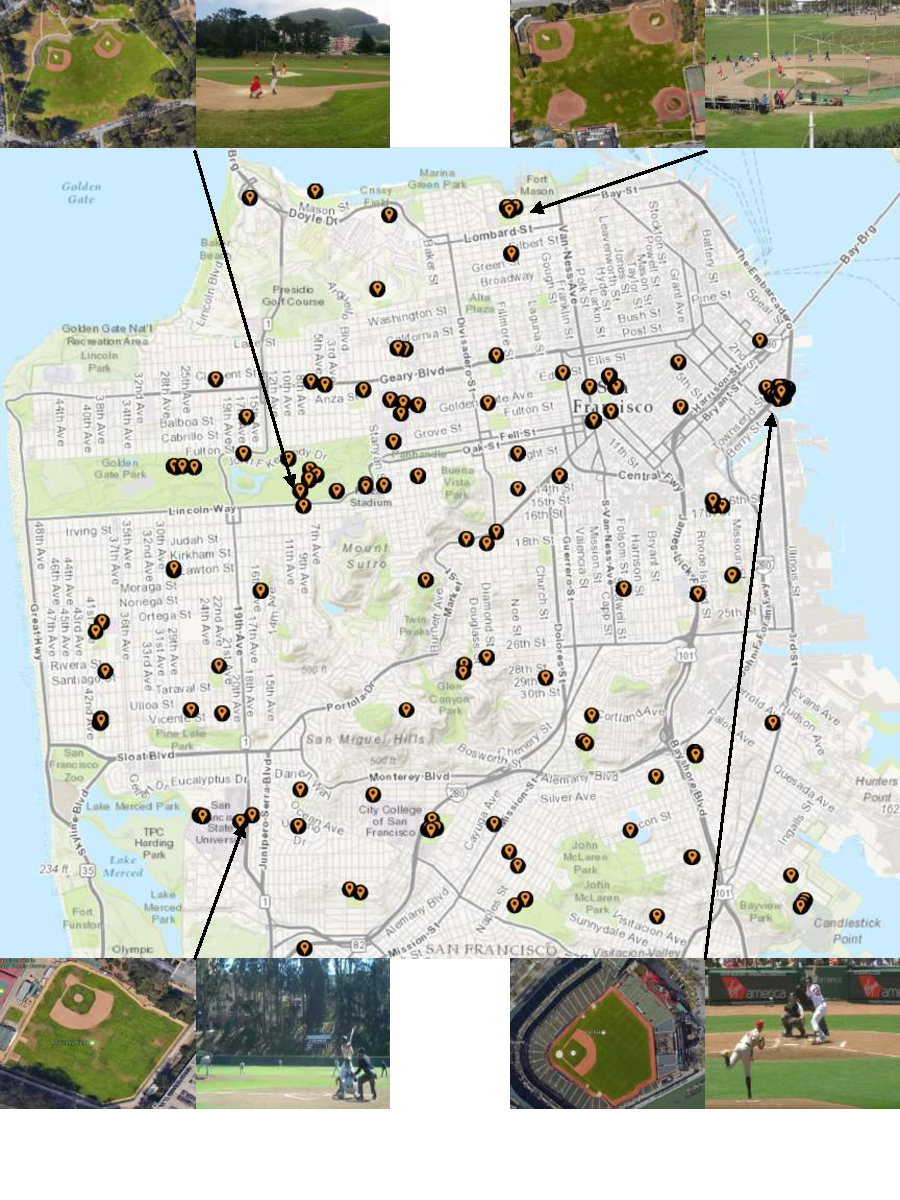
\includegraphics[width=0.32\linewidth,trim=0 25 0 0,clip]{baseball_youtube-min.pdf}\label{fig:baseball}}\hspace{1pt}
		\subfigure[Basketball]{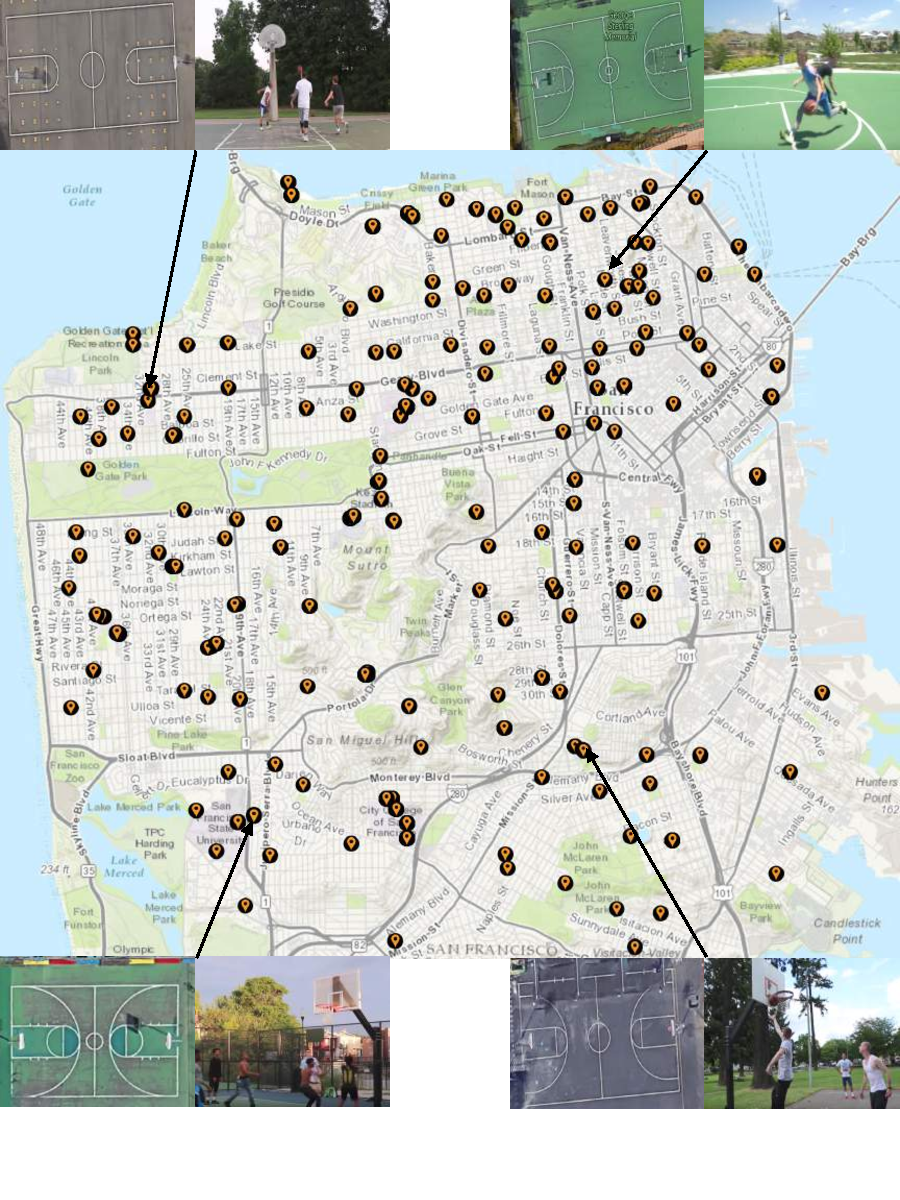
\includegraphics[width=0.32\linewidth,trim=0 25 0 0,clip]{basketball_youtube-min.pdf}\label{fig:basketball}}\hspace{1pt}
		\subfigure[Football]{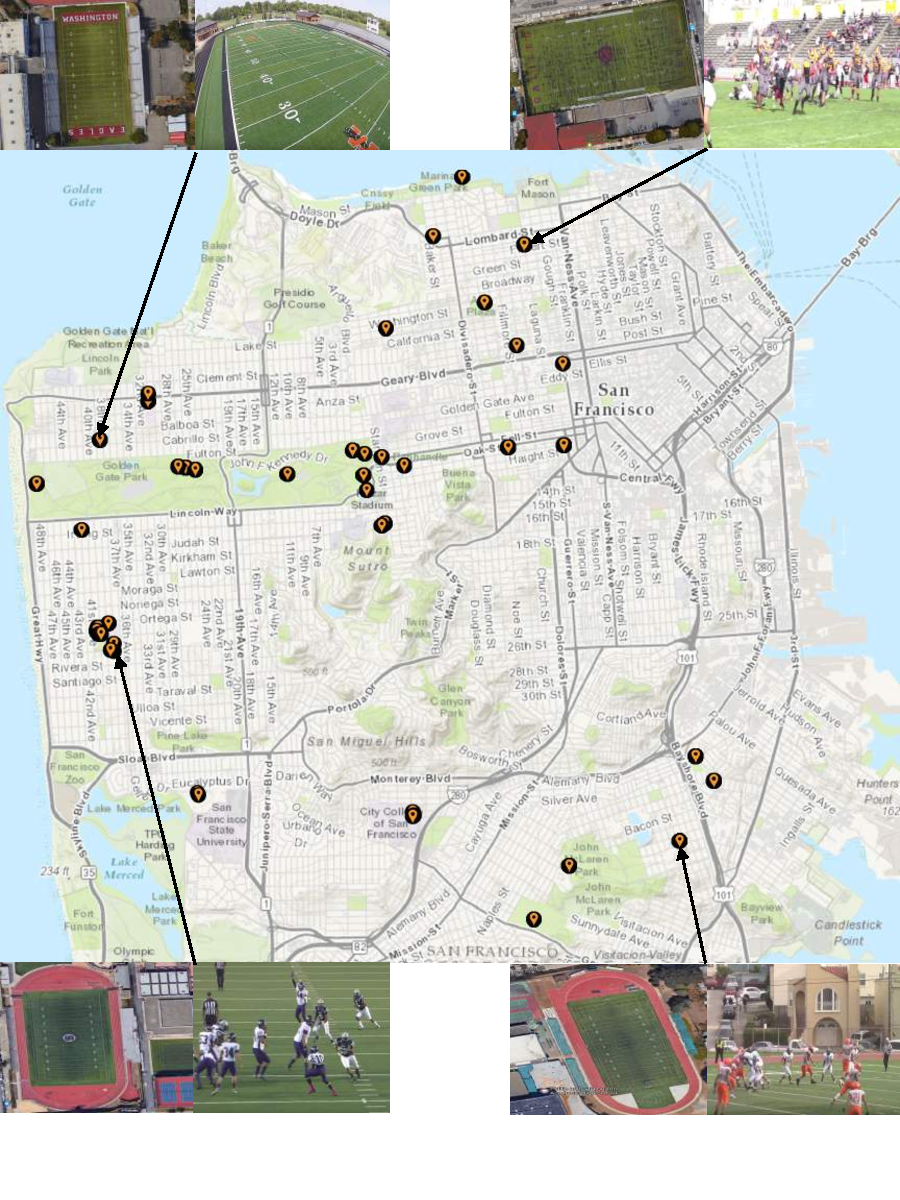
\includegraphics[width=0.32\linewidth,trim=0 25 0 0,clip]{football_youtube-min.pdf}\label{fig:football}}\hspace{1pt}
		\subfigure[Golf]{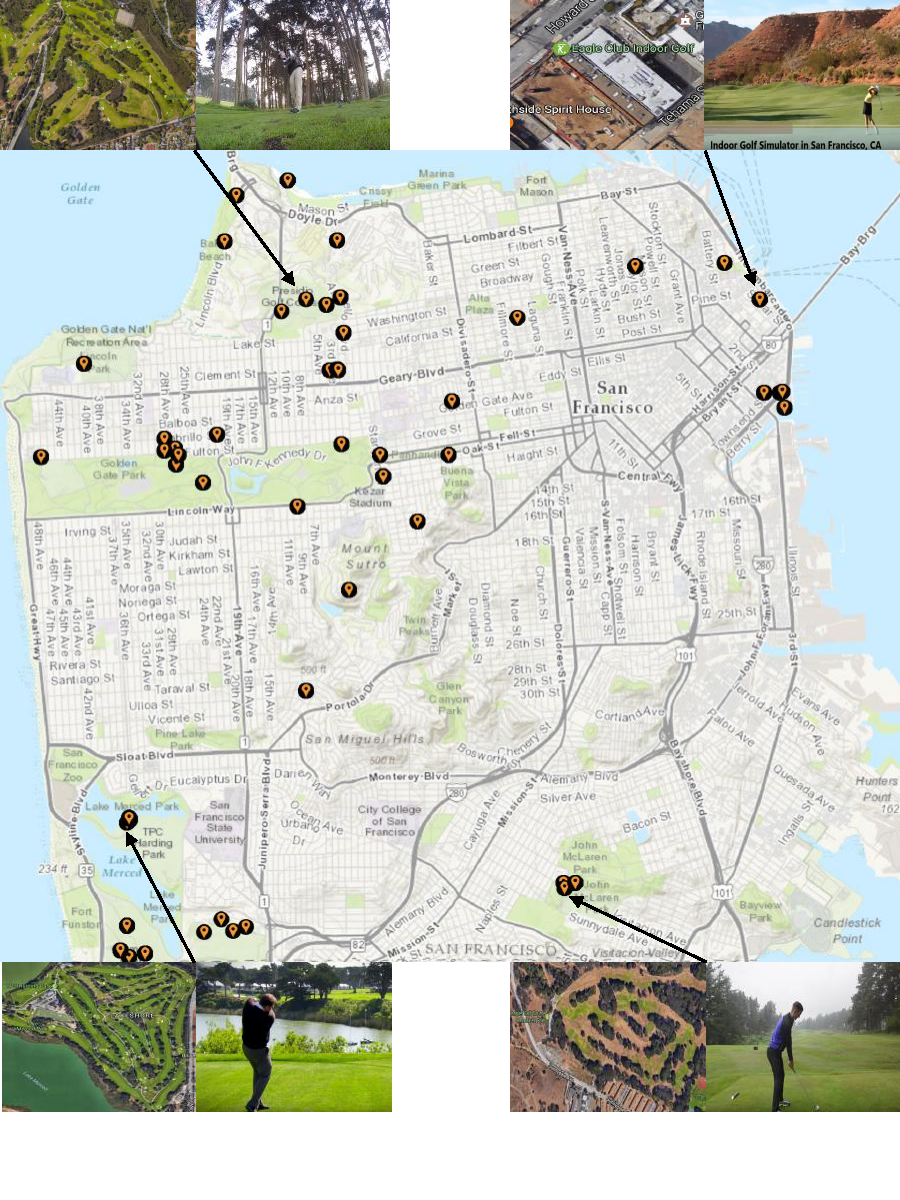
\includegraphics[width=0.32\linewidth,trim=0 25 0 0,clip]{golf_youtube-min.pdf}\label{fig:golf}}\hspace{1pt}
		\subfigure[Soccer]{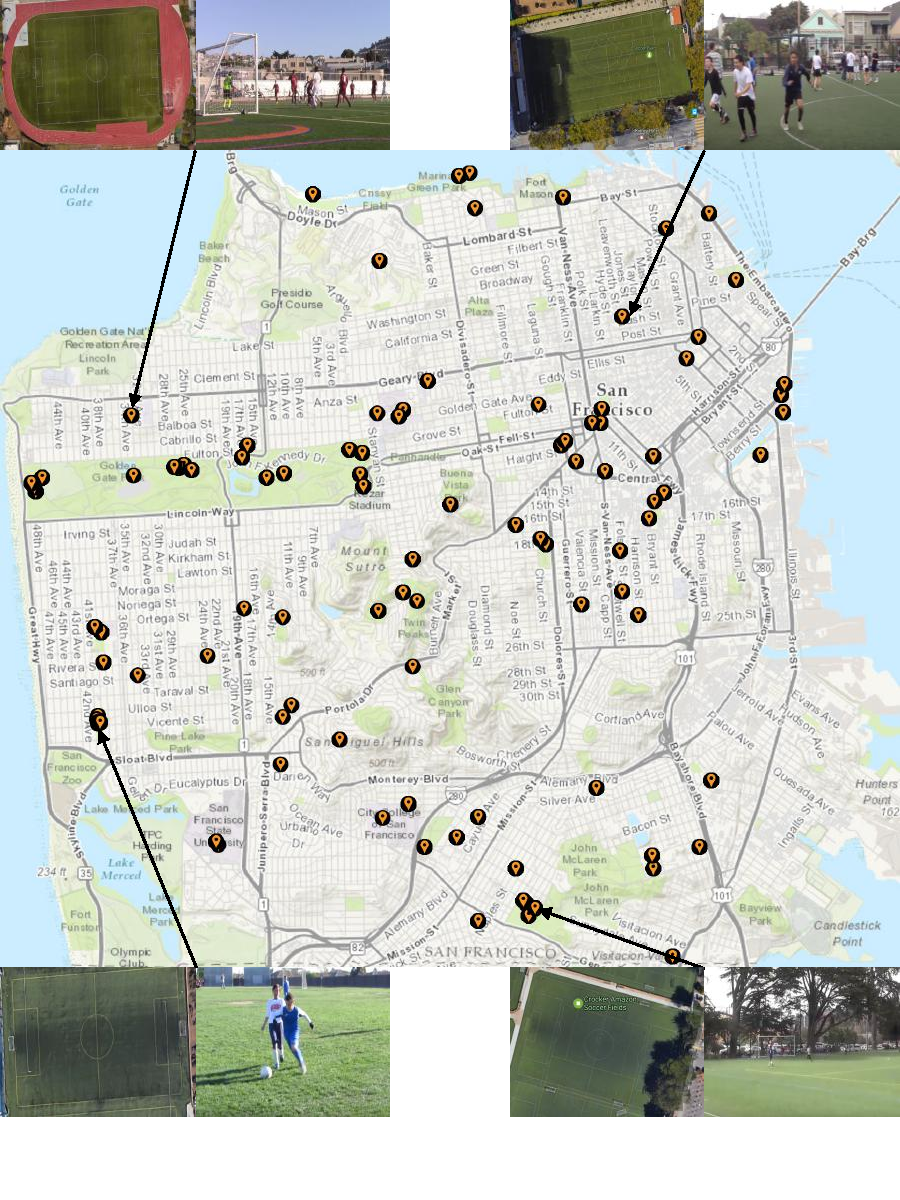
\includegraphics[width=0.32\linewidth,trim=0 25 0 0,clip]{soccer_youtube-min.pdf}\label{fig:soccer}}\hspace{1pt}
		\subfigure[Tennis]{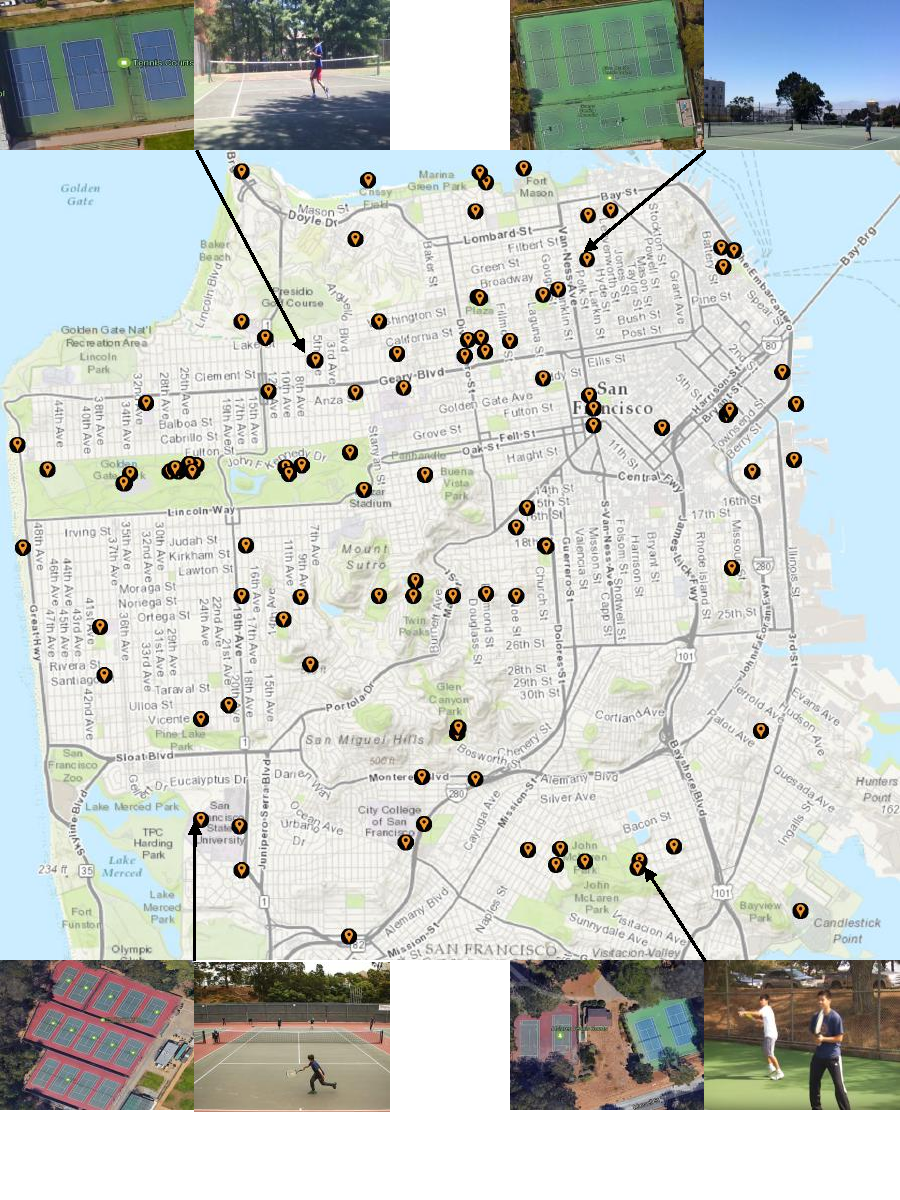
\includegraphics[width=0.32\linewidth,trim=0 25 0 0,clip]{tennis_youtube-min.pdf}\label{fig:tennis}}\hspace{1pt}
		\vspace{-1ex}
		\caption{这是译文 2016. (这是译文) 这是译文; (这是译文) 这是译文; (这是译文) 这是译文; (这是译文) 这是译文; (这是译文) 这是译文 (这是译文) 这是译文.}
		\label{fig:spatialActivityMap}
	\end{figure*}
	
	\begin{table}[t]
		\begin{center}
			\resizebox{0.8\columnwidth}{!}{%
				\begin{tabular}{ | c | c | c|}
					\hline
					Method										&    Accuracy (\%)  &    fps \\
					\hline
					C3D    					                    &   $84.57$ 	&    $390.7$\\
					Hidden Two-Stream CNNs     					&   $90.94$ 	&    $130.56$\\	
					\hline
					%				\hline
					%				C3D    					                    &   $76.13$ 	&    $390.7$\\	
					%				Hidden Two-Stream CNNs     					&   $83.26$ 	&    $130.56$\\	
					%				\hline
				\end{tabular}
			} 
			\vspace{2ex}
			\caption{这是译文. \label{tab:comparison}}
			\vspace{-4ex}
		\end{center}
	\end{table} 
	
	\begin{table}[t]
		\begin{center}
			\resizebox{0.6\columnwidth}{!}{%
				\begin{tabular}{ | c | c | c|}
					\hline
					Method										&    C3D (\%)   &    Hidden (\%) \\
					\hline
					Baseball    					           &   $86.57$ 	&    $90.29$\\
					Basketball    					           &   $88.62$ 	&    $94.43$\\
					Football    					           &   $85.14$ 	&    $88.63$\\
					Golf    					                &   $76.32$ 	&    $85.91$\\
					Racquetball    					           &   $88.90$ 	&    $92.11$\\
					Soccer    					                &   $83.49$ 	&    $89.43$\\
					Swimming    					           &   $92.27$ 	&    $97.51$\\
					Tennis    					                &   $80.19$ 	&    $84.60$\\
					Parade    					                &   $83.00$ 	&    $90.37$\\
					Street Fight    					           &   $81.20$ 	&    $96.12$\\
					\hline
					Mean Average    					           &   $84.57$ 	&    $90.94$\\
					\hline
				\end{tabular}
			} 
			\vspace{2ex}
			\caption{这是译文. \label{tab:break_down}}
			\vspace{-4ex}
		\end{center}
	\end{table} 
	
	\section{这是译文}
	\label{sec:experiments}  这是译文.
	
	\subsection{这是译文}
	\label{sec:dataset}  这是译文 $10$ 这是译文 \cite{KarpathyCVPR14}, 这是译文101 \cite{ucf101} 这是译文 \cite{FCVID} 这是译文\footnote{这是译文.} 这是译文 $10,000$ 这是译文, $1,000$ 这是译文101 \cite{ucf101} 这是译文 1.3 \cite{activityNet} 这是译文 $0.8$:$0.2$.
	
	这是译文 $2016$. 这是译文 $265,477$ 这是译文. 
	
	\subsection{这是译文}
	\label{sec:implementation}  这是译文 \cite{jia2014caffe} 这是译文7 (4.00这是译文) 这是译文. 
	
	\noindent \textbf{这是译文:}  这是译文 $L_{\text{pixel}}$, 这是译文 $L_{\text{smooth}}$ 这是译文 $L_{\text{ssim}}$. 这是译文 $\alpha$ 这是译文 $0.4$ 这是译文 $0.3$ 这是译文. 
	
	这是译文 $\beta_{1}=0.9$ 这是译文 $\beta_{2}=0.999$. 这是译文 $16$. 这是译文 $3.2\times10^{-5}$ 这是译文 $100$这是译文 $400$这是译文.
	
	\noindent \textbf{这是译文:}  这是译文 \cite{imagenet_cvpr09}, 这是译文 \cite{wanggoodpractice2015}. 这是译文 $128$ 这是译文 $0.9$.  这是译文.
	
	这是译文 $0.001$, 这是译文 $10$ 这是译文 $4$这是译文 $10$这是译文: $10^{-6}$ 这是译文 $10^{-3}$. 这是译文 $10$ 这是译文 $5$这是译文 $10$这是译文 $16$这是译文.
	
	\noindent \textbf{这是译文:}  这是译文 \cite{c3d2015} 这是译文 $3 \times 3 \times 3$ 这是译文 $2\times2\times2$ 这是译文 $1 \times 2 \times 2$. 这是译文 \cite{c3d2015} 这是译文.
	
	这是译文 $487$ 这是译文 (30 这是译文) 这是译文 (这是译文 0.9). 这是译文 $10^{-6}$. 这是译文 $0.7$ 这是译文.
	
	\subsection{这是译文}
	\label{sec:activity_recognition_evaluation}  这是译文 \ref{tab:comparison} 这是译文 $90\%$ 这是译文 $6\%$ 这是译文 (30 这是译文). 
	
	这是译文 \ref{tab:break_down} 这是译文 (这是译文) 这是译文.
	
	这是译文.
	
	\begin{figure}[t]
		\centering
		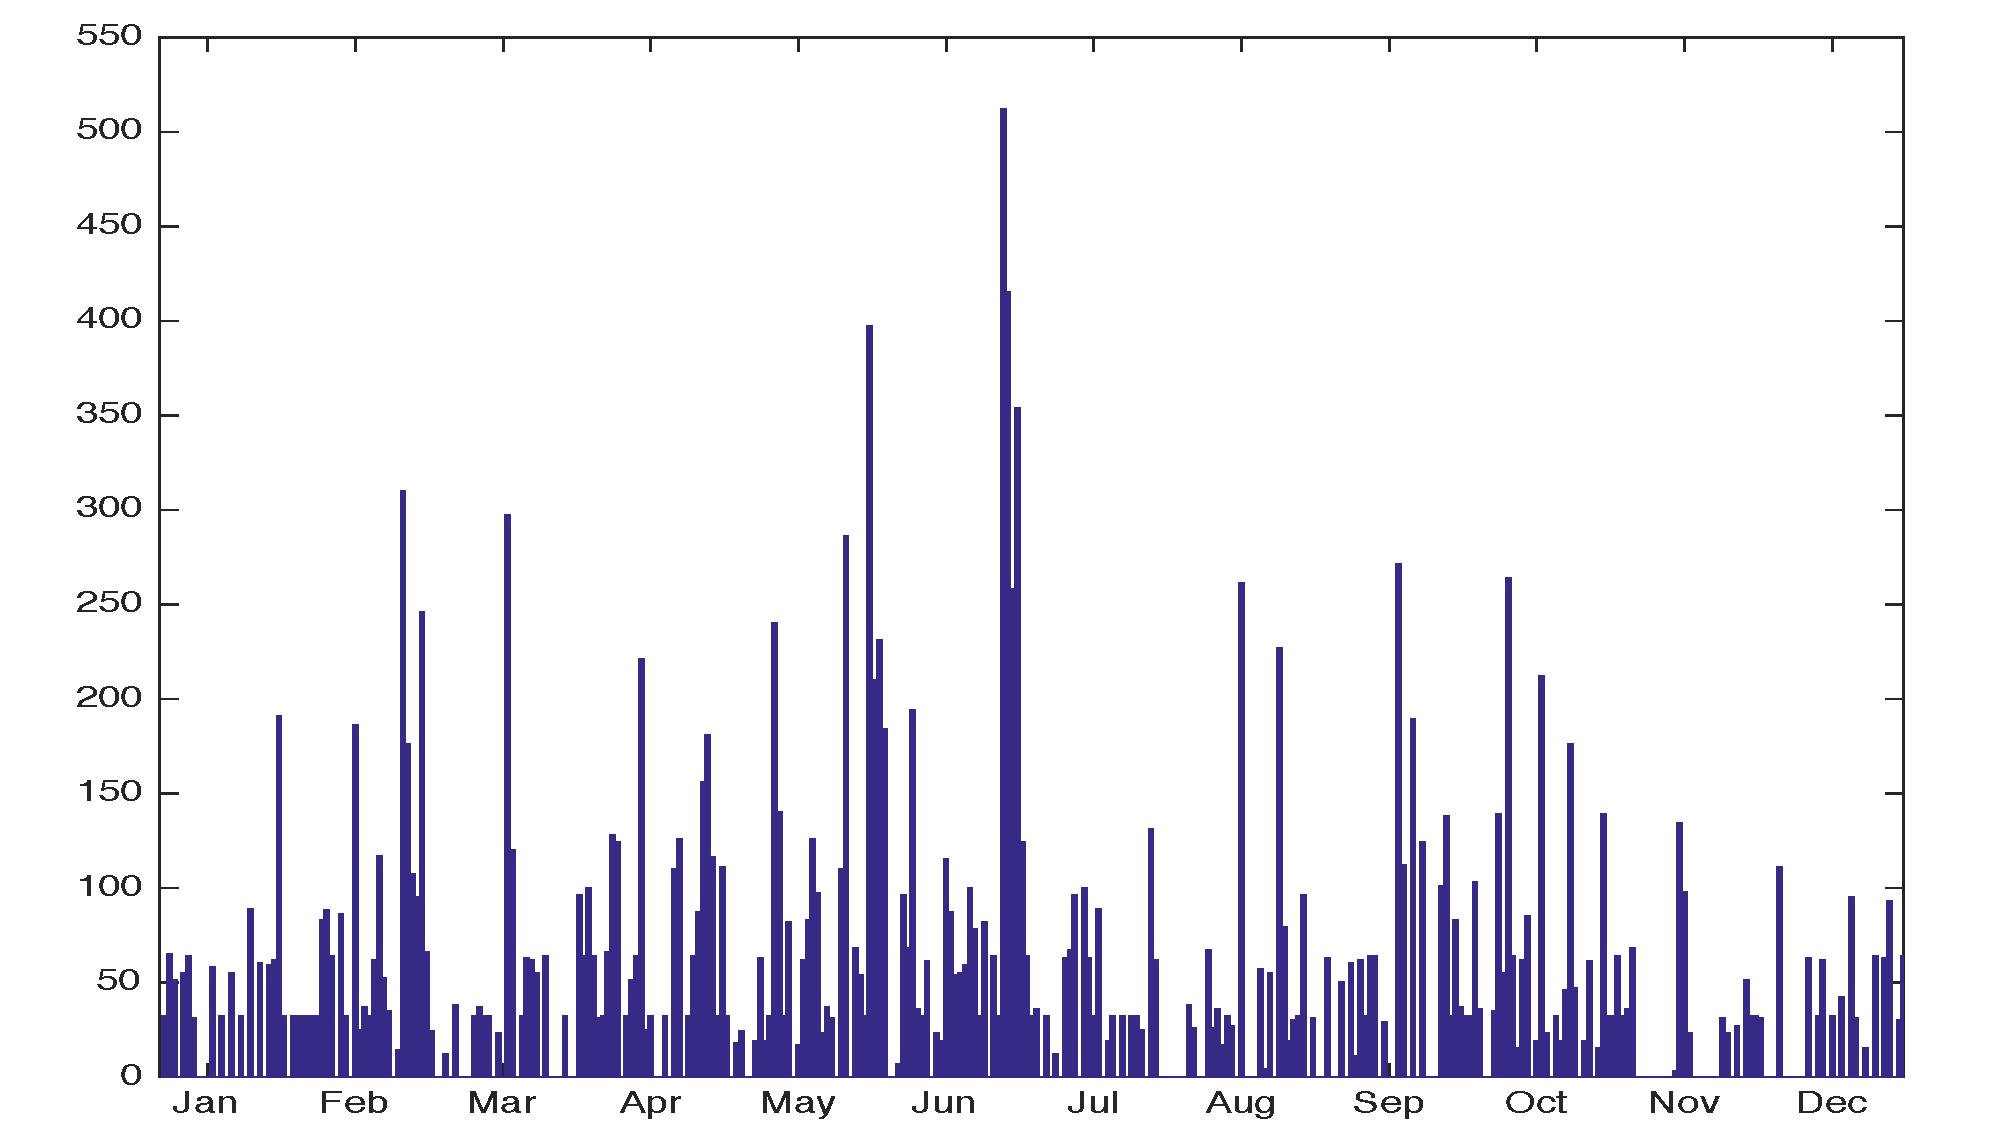
\includegraphics[width=1.0\linewidth,trim=0 0 0 0,clip]{parade_temporal.pdf}
		\caption{这是译文.}
		\label{fig:parade_temporal}
		% \vspace{-3ex}
	\end{figure}
	
	\begin{figure}[t]
		\centering
		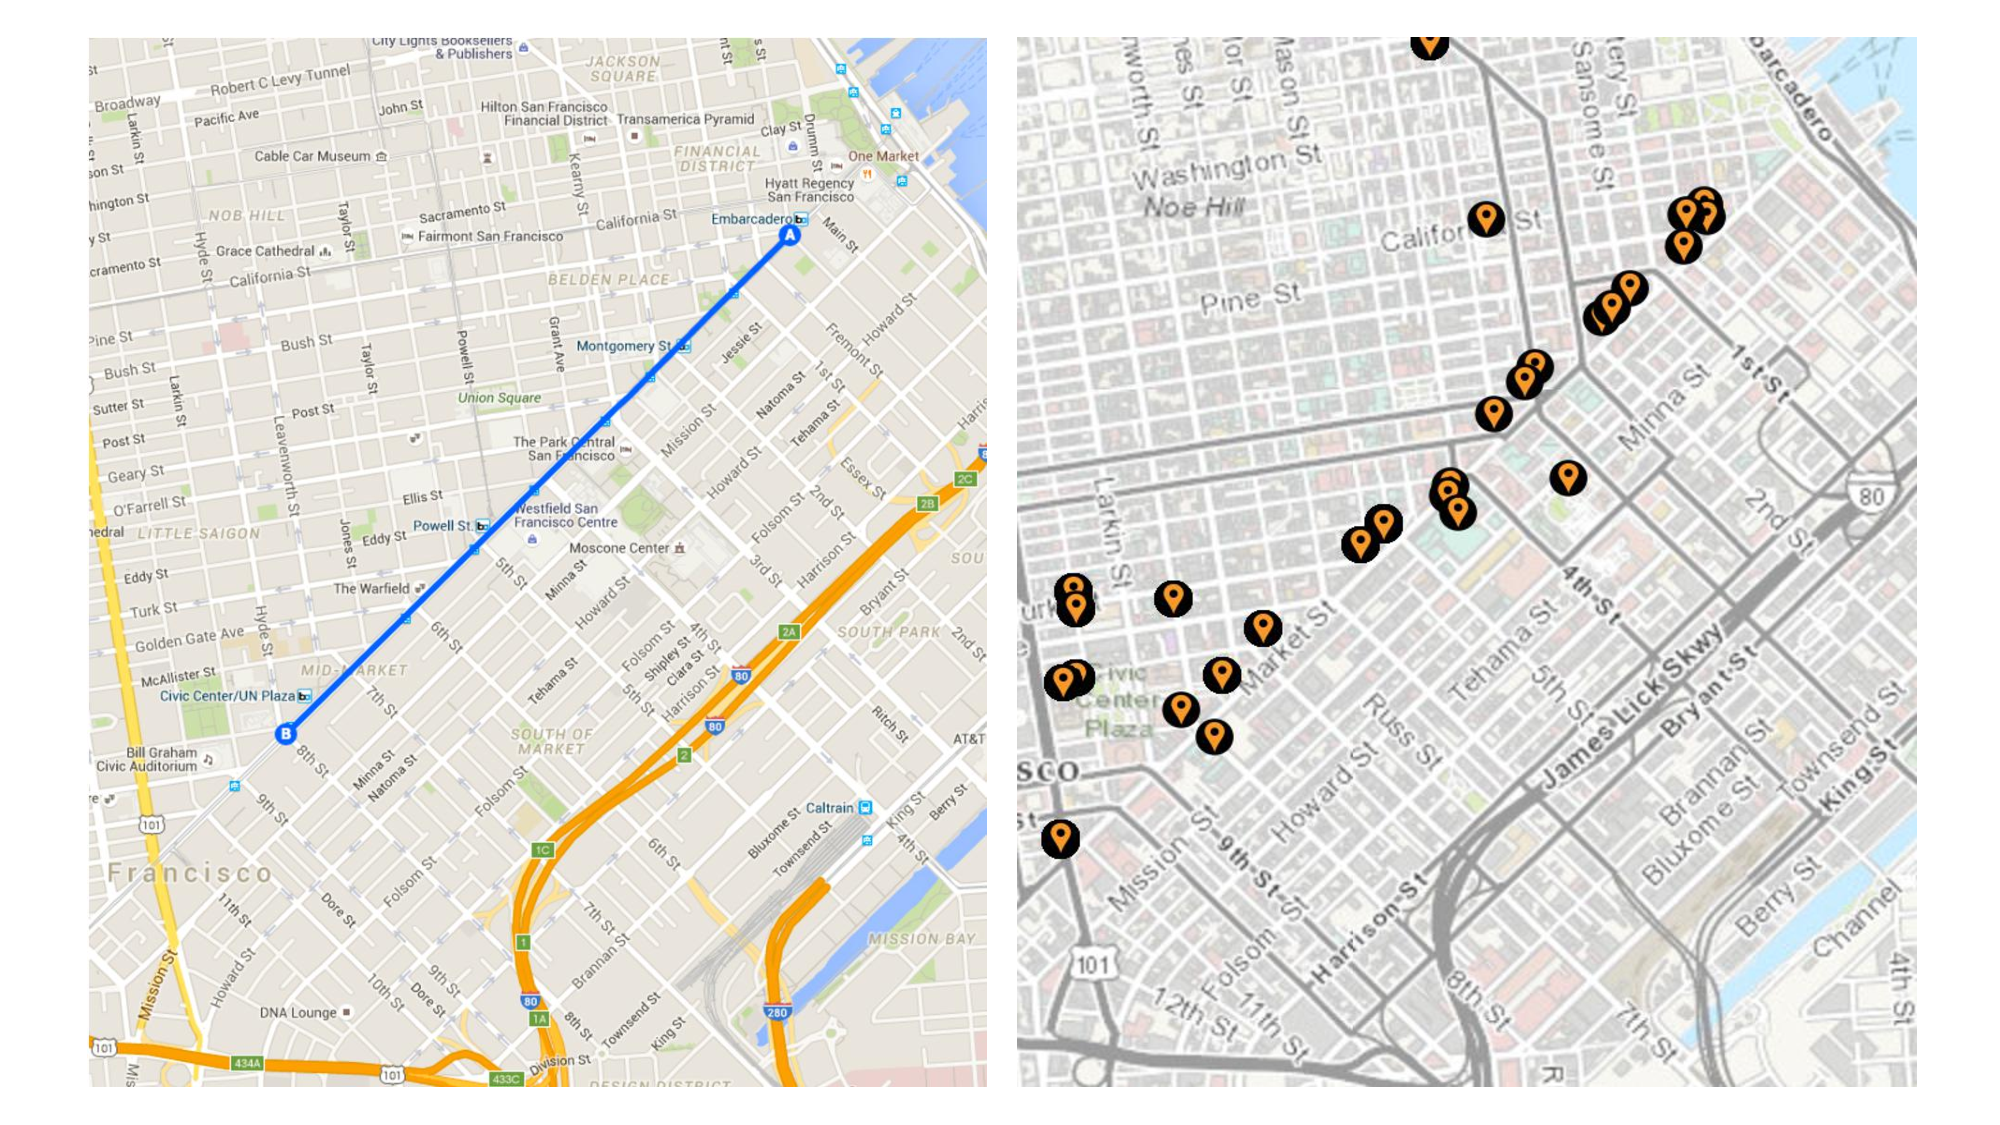
\includegraphics[width=1.0\linewidth,trim=0 0 0 0,clip]{parade_spatial-min.pdf}
		\caption{这是译文.}
		\label{fig:parade_spatial}
		%\vspace{-2ex}
	\end{figure}
	
	\subsection{这是译文}
	\label{sec:spatial_sports_mapping}  这是译文 \ref{fig:spatialActivityMap} 这是译文) 这是译文) 这是译文.
	
	这是译文 \ref{fig:spatialActivityMap}.
	
	\noindent \textbf{这是译文 1}: 这是译文 \ref{fig:baseball} 这是译文$\&$这是译文. 
	
	这是译文.
	
	%Most of the videos are mapped correctly despite some noisy data. For example, lots of the basketball videos are shown in the high density residential area instead of a basketball court. We perform a sanity check of all those videos and found that some of those videos are indeed shoot in the home or backyard (which means the auto-labelling and mapping is correct), while some other videos are just wrongly geo-tagged (which represents the noisy geo-tag problem in using YouTube videos for geographic knowledge discovery).
	
	\noindent \textbf{这是译文 2}: 这是译文.
	
	%The amount of geo-tagged videos for golf and football are much fewer than the other activity categories. It makes sense for golf since playing golf require a professional field and a good weather. But it is counter-intuitive for football as football is one of the most popular sports in United States. 
	%After a sanity check into our training set, we found the reason maybe because most football videos in the Sports1M dataset is captured during matches. Thus people playing football without helmet and suit is hard to recognize. Besides, the amount of players, the environment also differs a lot between the training data and test data, which leads to fewer detection on the map. We believe with more diverse geo-tagged videos as training data and advanced data augmentation technique, our model can generalize well. 
	
	\noindent \textbf{这是译文 3}: 这是译文 (这是译文 \ref{fig:golf}) 这是译文.
	
	\noindent \textbf{这是译文 4}: 这是译文 \ref{fig:football}, 这是译文 \ref{fig:soccer}, 这是译文.
	
	\subsection{这是译文}
	\label{sec:spatio_temporal_parade_mapping}  这是译文.
	
	\noindent \textbf{这是译文}: 这是译文 $15,645$ 这是译文 \ref{fig:parade_temporal}. 这是译文 (这是译文 20), 这是译文 (这是译文 12), 这是译文 (这是译文 28), 这是译文 (这是译文 25) 这是译文 (这是译文 9).
	
	这是译文.
	
	%There is another observation that people usually upload relevant videos after the event, sometimes even several days later. This observation is unique for videos, because texts or pictures are often shared immediately during the event. The reason for this is possibly because video is still too large for people to share when there is no Wifi. And sometimes people prefer to upload the video after serious video editing. 
	
	\noindent \textbf{这是译文}: 这是译文 2016 (这是译文), 这是译文 \ref{fig:parade_spatial}, 这是译文 (这是译文) 这是译文 (这是译文), 这是译文.
	
	%As the 46th Pride parade is the most popular parade in San Francisco last year ($512$ videos in a single day), we pick it as an example and map the videos spatially to see where the parade happens. As shown in Figure \ref{fig:parade_spatial}, our mapping results (right) corresponds well to the official parade route (left), from Market/Beale to Market/8th Street in downtown San Francisco. The points of interest are sparse because the number of geo-tagged videos are too small for mapping in such a large area. With more and more geo-tagged videos uploaded to YouTube, the mapping results would be more promising. 
	
	%Though many previous literature have done such spatio-temporal analysis using Twitter or Instagram, to our best knowledge, this is the first work to use videos and content-based video classification technique to do geographic knowledge discovery.
	
	\begin{figure}[t]
		\centering
		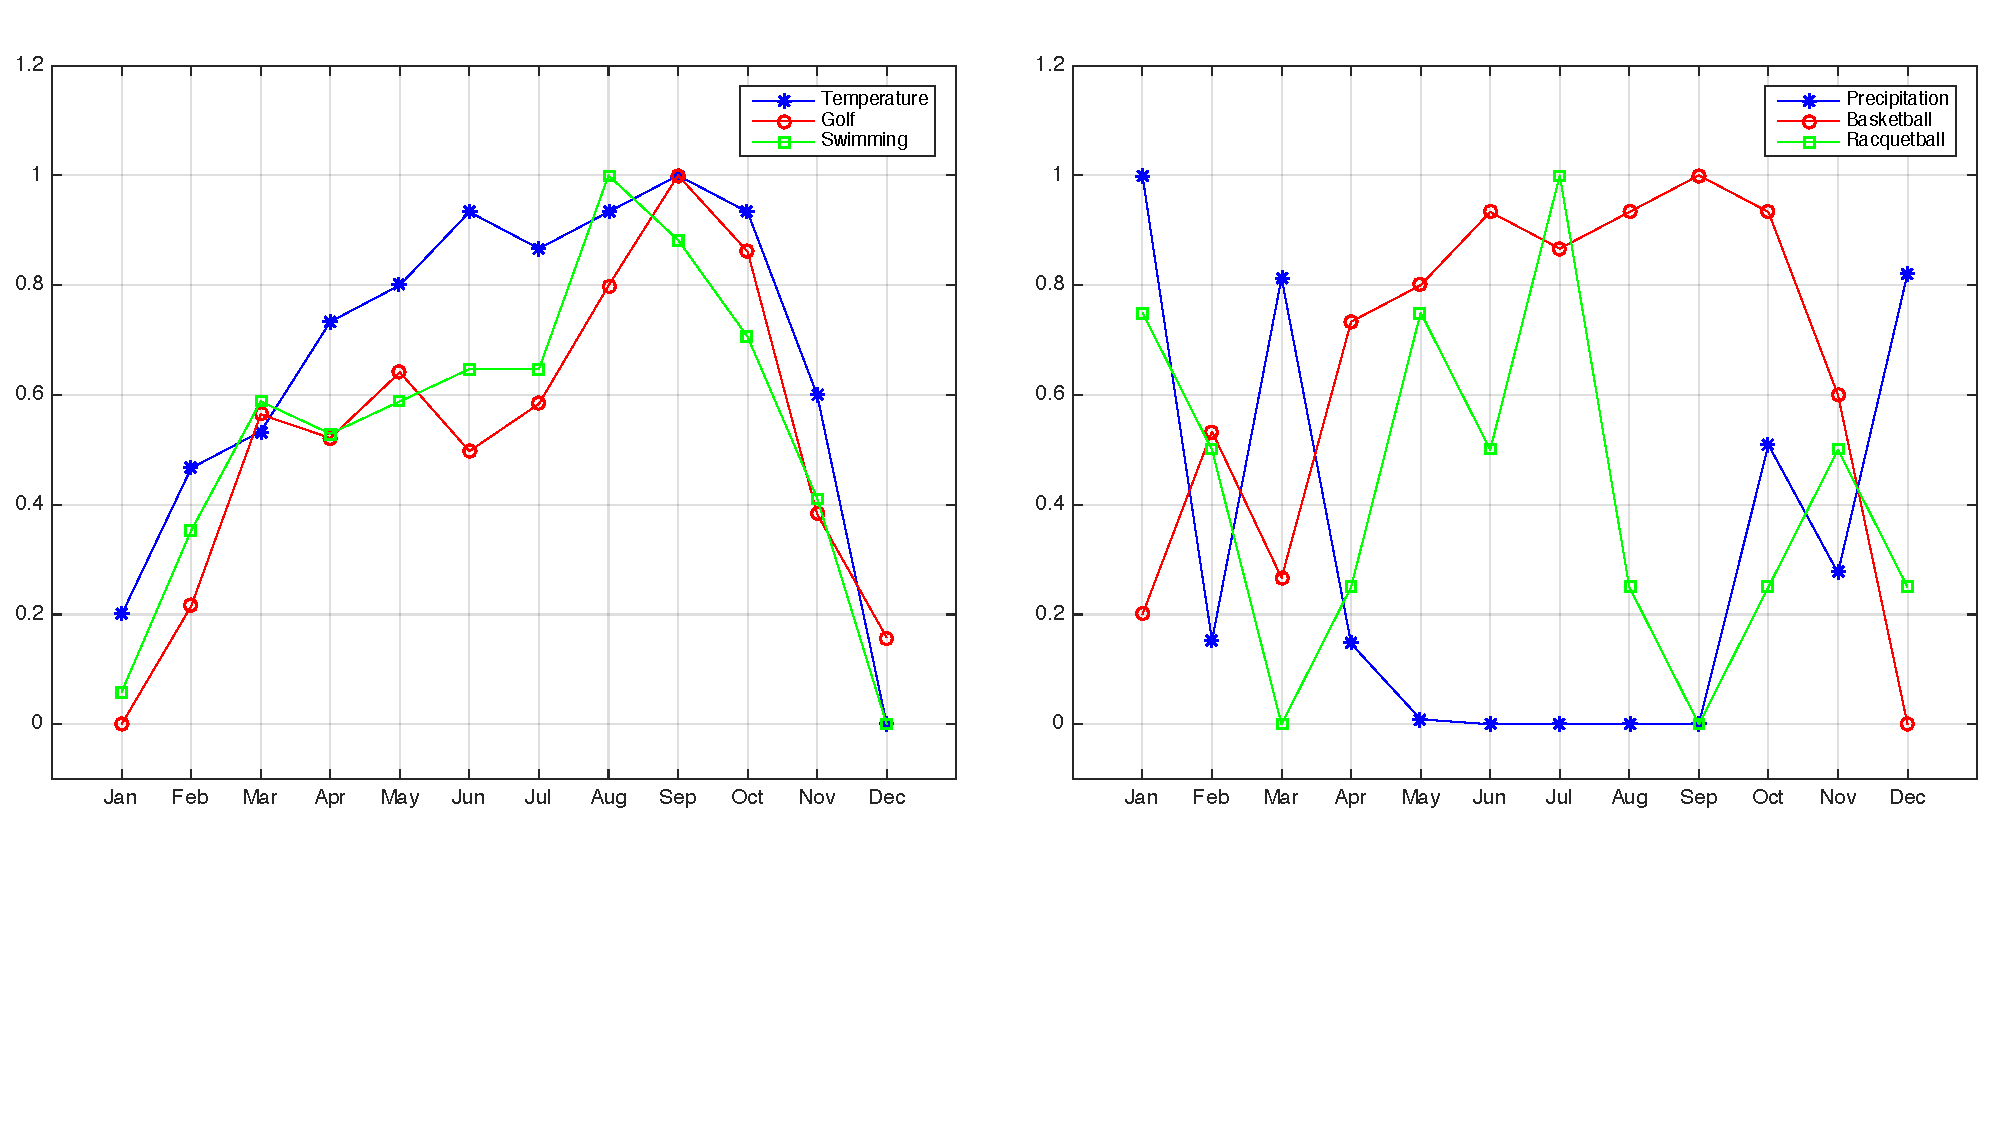
\includegraphics[width=1.0\linewidth,trim=0 0 0 0,clip]{weather.pdf}
		\vspace{-12ex}
		\caption{这是译文.}
		\label{fig:weather}
		\vspace{-2ex}
	\end{figure}
	
	\subsection{这是译文}
	\label{sec:weather_impact_on_human_activities}  这是译文\footnote{这是译文/.}. 这是译文 $0\sim1$ 这是译文.
	
	%For human activeness, we use the number of geo-tagged videos as a metric. Due to different scale of temperature, precipitation and number of videos, we normalize them to the range of $0\sim1$ for better visualization.
	
	\noindent \textbf{这是译文}: 这是译文 \ref{fig:weather} 这是译文.
	
	%When the temperature is lower in Winter, the activities are less frequently uploaded on YouTube. This makes sense because most people prefer to play golf or go to swimming in warm days. 
	
	\noindent \textbf{这是译文}: 这是译文 \ref{fig:weather} 这是译文 (这是译文) 这是译文 (这是译文) 这是译文.
	
	%Actually, the number of geo-tagged videos for racquetball is quite stable across the whole year. The reason why it fluctuates in Figure \ref{fig:weather} is because of the $0\sim1$ normalization. 
	
	% \subsection{Large-Scale Sports Preference}
	% Maybe wait for the journal version, I don't have time and computing resources to do country-level experiments. There are much more videos than I think there was. 
	\begin{figure}[t]
		\centering
		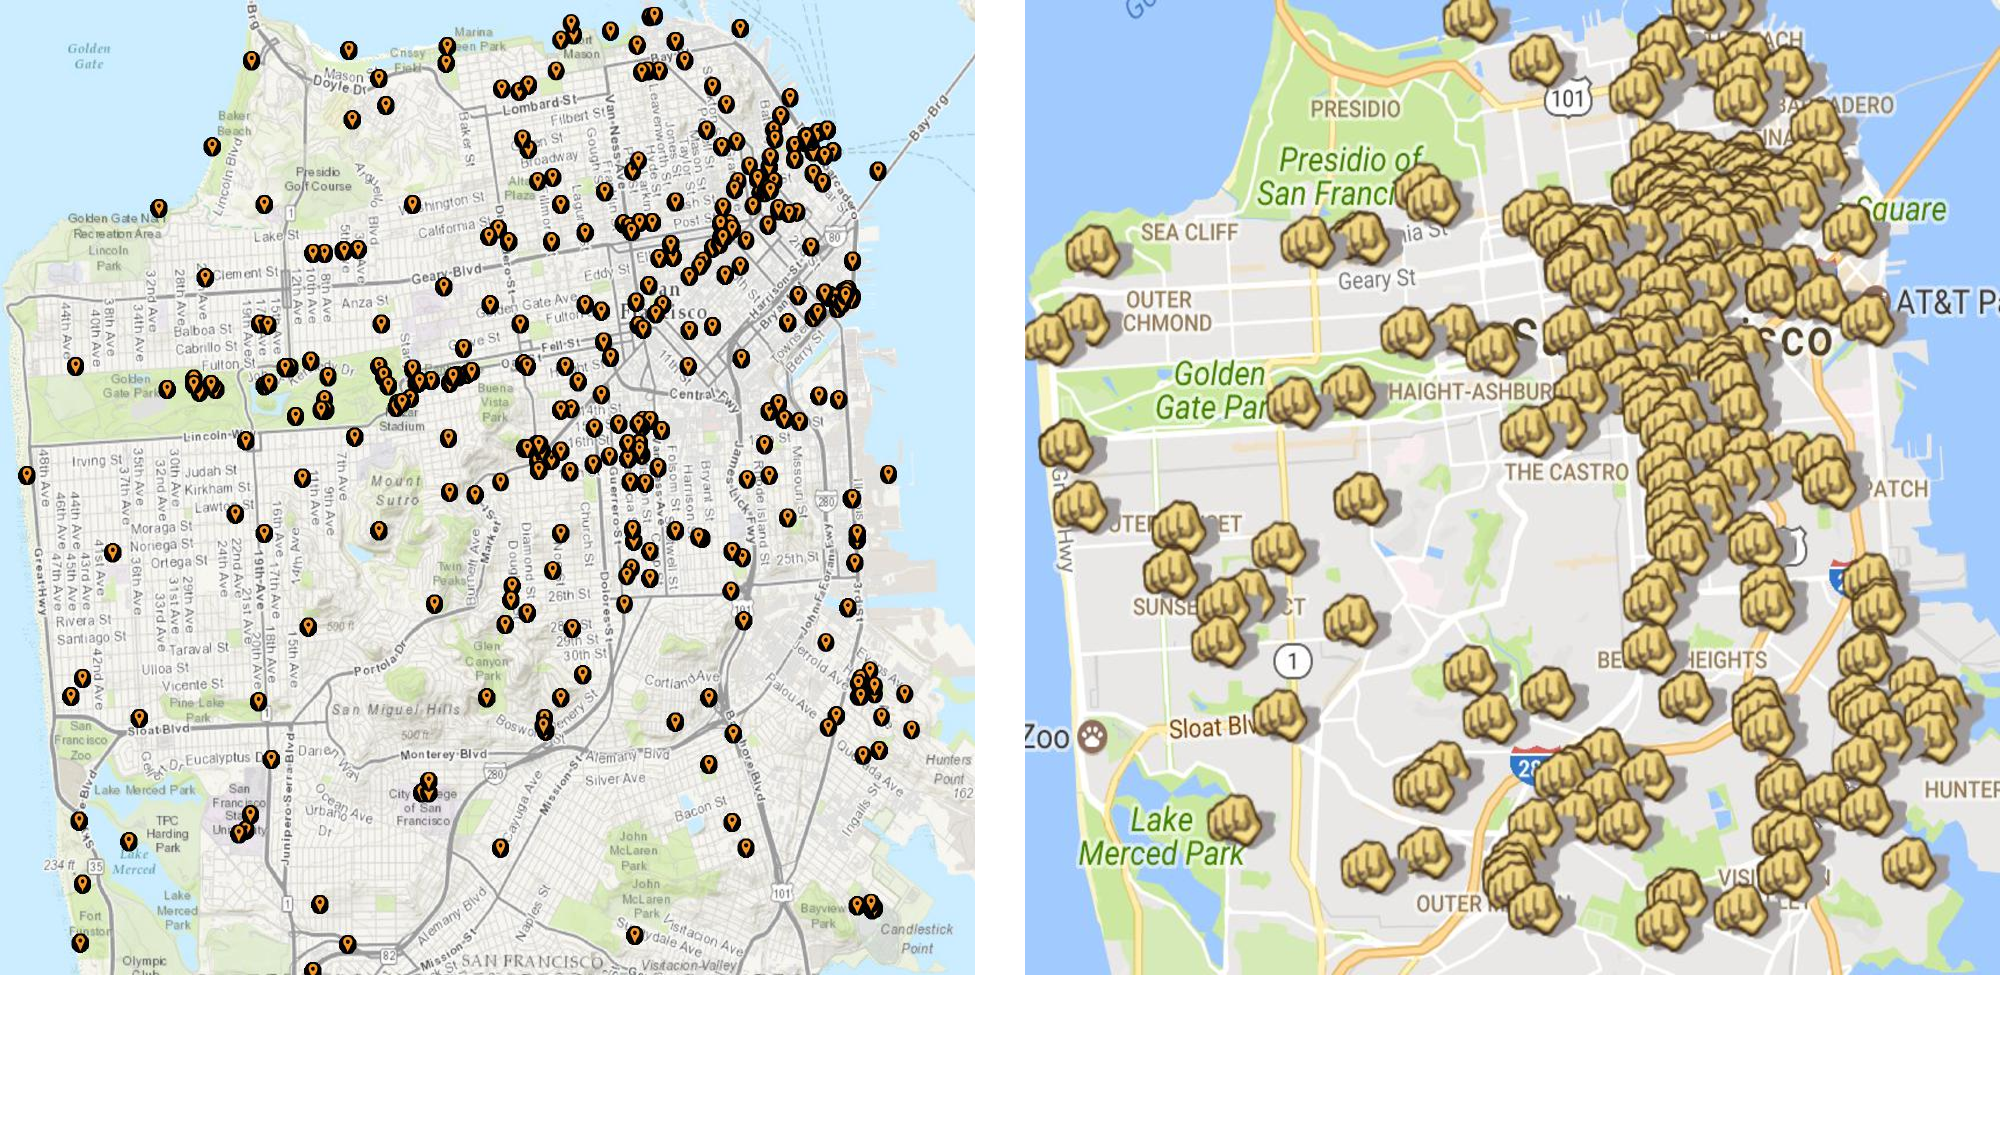
\includegraphics[width=1.0\linewidth,trim=0 0 0 0,clip]{street_fight-min.pdf}
		\vspace{-6ex}
		\caption{这是译文.}
		\label{fig:street_fight}
		\vspace{-2ex}
	\end{figure}
	
	\subsection{这是译文}
	\label{sec:violence_detection}
	
	这是译文.
	
	这是译文 $7,784$ 这是译文 \ref{fig:street_fight} 这是译文 \ref{fig:street_fight} 这是译文\footnote{这是译文} 这是译文.
	
	这是译文.
	
	%As we mentioned in Section \ref{sec:introduction}, our framework is flexible. We can adapt to other application scenarios using the same pipeline as long as there exists enough geo-tagged videos. For example, violence detection is a crucial component in monitoring social security. Although the government deployed millions of video cameras, it is impossible for human to watch those surveillance videos and report suspicious activities. Only machine vision can. 
	
	%In this work, we use YouTube videos as the data source and try to detect activity ``street fight'' from them. After auto-labeling, our model predict a total of $7,784$ street fight videos. The mapping result can be seen in Figure \ref{fig:street_fight} left. We notice several concentration of violence in Downtown San Francisco, Mission District, Hunters Point, etc. In order to show our method's effectiveness, we borrowed the San Francisco crime map (Figure \ref{fig:street_fight} right) \footnote{Data source is from: https://spotcrime.com/ca/san+francisco} and compare to our street fight geo-visualizations. Note that, we only map the ``Assault'' incidents because it is close to street fight. In fact, the street fight mapping is very similar to the assault mapping from official police records. This demonstrate that with our model and unlimited geo-tagged videos, we can detect and report violence in real-time as well as in large-scale. 
	
	\begin{figure}[ht]
		\centering
		\subfigure[Tag/Title Based Method]{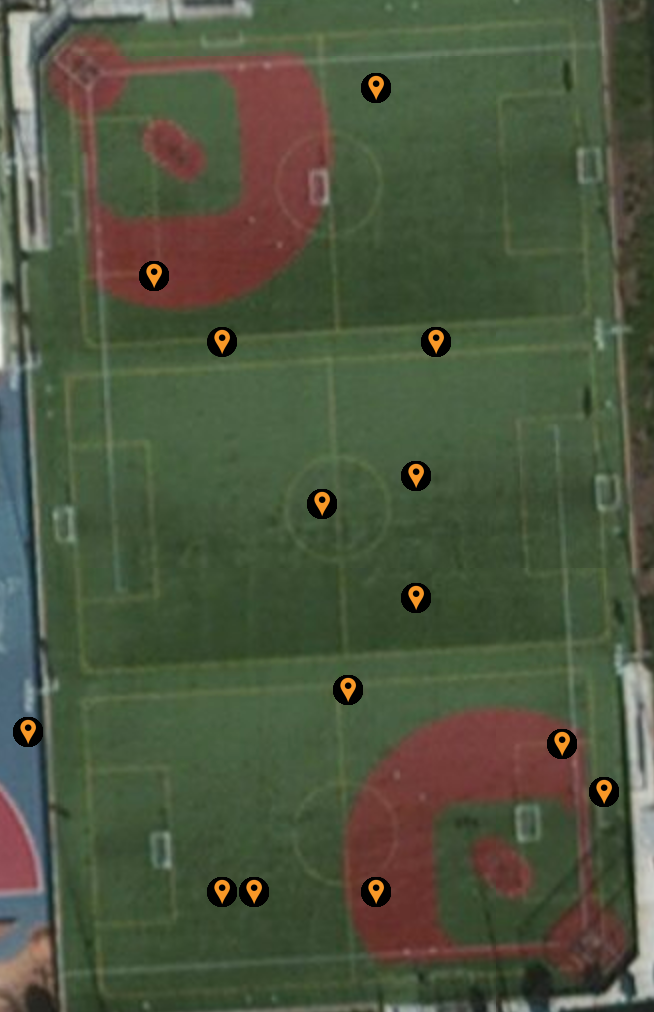
\includegraphics[width=0.45\linewidth,trim=0 0 0 0,clip]{football_soccer_false.png}\label{fig:football_soccer_false}}\hspace{2pt}
		\subfigure[Content Based Method (ours)]{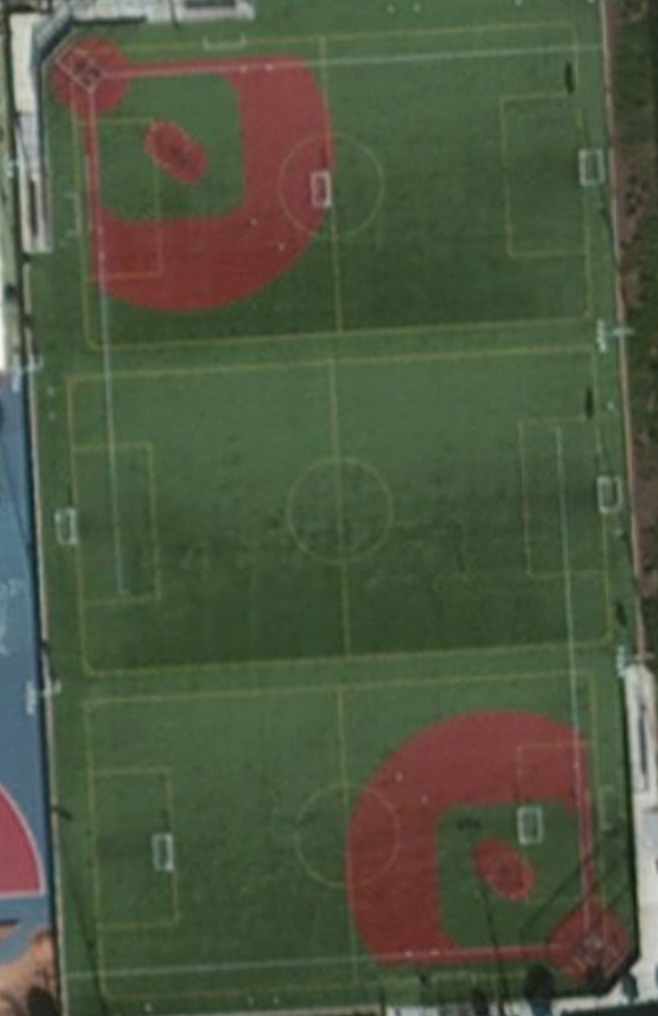
\includegraphics[width=0.45\linewidth,trim=0 0 0 0,clip]{football_soccer.png}\label{fig:football_soccer}}\hspace{0pt}
		\vspace{-2ex}
		\caption{这是译文.}
		\label{fig:content_advantage}
	\end{figure}
	
	\section{这是译文}
	\label{sec:discussion}
	
	\noindent \textbf{这是译文}
	
	这是译文.  
	
	这是译文 \ref{fig:content_advantage} 这是译文.
	
	%As can be shown in Figure \ref{fig:content_advantage}, this is a soccer field in the Ulloa elementary school in San Francisco sunset district. But due to wrong tags/titles (like ``football campaign'', ``kids playing football''), there are lots of videos mapped here as football as shown in Figure \ref{fig:football_soccer_false}.  However, our content-based model report nothing here as can be seen in Figure \ref{fig:football_soccer}. This clearly demonstrate that content-based method is more accurate than tag/title-based system. This finding is also observed in other geographic research areas, like land use land cover classification. 
	
	
	%Traditional approaches for mapping detailed human activities use video tags/titles to determine the category and then map it. This line of method is good due to its efficiency because the tags/titles are provided by users and can be obtained free of charge. At the same time, the tags/titles are correct or at least relevant in most cases. 
	%But if we come across missing tags/titles, or the tags/titles don't contain useful information or even wrong information, those approaches would fail completely. 
	
	%The advantage of using activity recognition model to auto-label YouTube videos over tag/title based system is: the predicted activity category solely depends on the video content, and won't be confused by other information, like the metadata.  
	
	%Take mapping football and soccer as an example. In some other countries, people often refer soccer as football as well. Thus, when these users upload a video to YouTube, it is highly likely that the tags/titles are wrong with respect to the video content. As can be shown in Figure \ref{fig:content_advantage}, this is a soccer field in the Ulloa elementary school in San Francisco sunset district. But due to wrong tags/titles (like ``football campaign'', ``kids playing football''), there are lots of videos mapped here as football as shown in Figure \ref{fig:football_soccer_false}.  However, our content-based model report nothing here as can be seen in Figure \ref{fig:football_soccer}. This clearly demonstrate that content-based method is more accurate than tag/title-based system. This finding is also observed in other geographic research areas, like land use land cover classification. 
	
	\section{这是译文}
	\label{sec:conclusion}  这是译文.
	
	这是译文.
	
	这是译文.
	
	
	%We conduct the first investigation into using geo-tagged videos to do human activity mapping and analysis. We propose a fast video analysis method for action recognition, named hidden two stream networks. The model can run at a speed of $130$ fps, which enables real-time applications. Besides, it can achieve more than 90 percent accuracy on a $10$ class activity classification problem. We also showcase some applications with spatio-temporal analysis. We spatially show that our activity recognition model can effective label YouTube videos into different activity categories. Then we temporally show the impact of weather onto different human activities. Through spatio-temporal analysis, our method can locate specific events such as parading and street fight. All expriments demonstrate the accuracy, efficiency and flexible of our method. 
	
	%For future work, we want to adapt our approach to surveillance videos and predict suspicious activities, like stealing, crowding etc, and use it for public safety monitoring. Surveillance videos and YouTube videos are quite different in terms of image quality, viewpoint, and camera motion. Another interesting line of research is to perform even larger-scale geographic knowledge discovery, like country-scale or global scale. Also, the number of activity categories should be scaled up. In addition, we want to shrink our model size using binarized or hashing technique to fit our algorithm on mobile or embedded platforms. We can directly analyze videos at endpoint equipment, like IP cameras. In this case, we don't need to upload the video to cloud in order to use advanced deep learning technology. 
	
	
	\section{这是译文}
 这是译文, \#这是译文 (这是译文).
	
	
	\bibliographystyle{ACM-Reference-Format}
	\input{sample-sigconf.bbl} 
	
\end{document}
